\documentclass[aspectratio=169]{beamer}

\usepackage[utf8]{inputenc}
\usepackage[T1]{fontenc}
\usepackage{graphicx}
\usepackage{tikz}
\usetikzlibrary{shapes.geometric, arrows.meta, positioning, calc}
\usepackage{pgfplots}
\pgfplotsset{compat=1.18}
\usepackage{booktabs}
\usepackage{colortbl}
\usepackage{amsmath}
\usepackage{siunitx}
\sisetup{detect-all}

\usetheme{Madrid}
\usecolortheme{default}

\definecolor{primary}{RGB}{0,102,153}
\definecolor{accent}{RGB}{230,159,0}
\definecolor{success}{RGB}{0,158,115}
\definecolor{danger}{RGB}{213,94,0}

\setbeamercolor{structure}{fg=primary}
\setbeamercolor{palette primary}{bg=primary,fg=white}
\setbeamercolor{palette secondary}{bg=primary!80,fg=white}
\setbeamercolor{palette tertiary}{bg=primary!60,fg=white}
\setbeamercolor{frametitle}{bg=primary,fg=white}
\setbeamercolor{title}{fg=primary}
\setbeamercolor{block title}{bg=primary,fg=white}
\setbeamercolor{block body}{bg=primary!5,fg=black}

\setbeamertemplate{navigation symbols}{}
\setbeamertemplate{footline}{
  \leavevmode%
  \hbox{%
    \begin{beamercolorbox}[wd=.333333\paperwidth,ht=2.25ex,dp=1ex,center]{author in head/foot}%
      \usebeamerfont{author in head/foot}\insertshortauthor
    \end{beamercolorbox}%
    \begin{beamercolorbox}[wd=.333333\paperwidth,ht=2.25ex,dp=1ex,center]{title in head/foot}%
      \usebeamerfont{title in head/foot}\insertshorttitle
    \end{beamercolorbox}%
    \begin{beamercolorbox}[wd=.333333\paperwidth,ht=2.25ex,dp=1ex,right]{date in head/foot}%
      \usebeamerfont{date in head/foot}
      \insertframenumber{} / \inserttotalframenumber\hspace*{2ex}
    \end{beamercolorbox}}%
  \vskip0pt%
}

\graphicspath{{../models/plots/}{./}}

\title[Multi-Modal Hand Gesture]{A Vision-First Multi-Modal Approach\\for Hand Gesture Recognition}
\subtitle{Interactive Puzzle Game Control via Skeleton \& Appearance Methods}
\author[Hieu, Nhat Anh, Quoc Anh]{Hieu Dinh \and Nhat Anh \and Quoc Anh}
\institute{Computer Vision Course}
\date{\today}

\begin{document}

% ======== 1. TITLE ========
\begin{frame}[plain]
    \titlepage
\end{frame}


% ======== 2. RESEARCH QUESTIONS ========
\begin{frame}{Research Questions \& Pipeline}
    \vspace{0.5em}

    \begin{block}{Core Question}
        \centering
        Does fusing \textbf{skeleton} (geometric) and \textbf{appearance} (visual) features\\
        from a single RGB camera improve hand gesture recognition?
    \end{block}

    \vspace{0.8em}
    \begin{columns}[T]
        \begin{column}{0.48\textwidth}
            \textbf{Q1 (Multi-Modal):} How do methods of increasing complexity compare? Does fusion add value?

            \vspace{0.6em}
            \textbf{Q2 (Deployment):} What is the \textit{lightest model sufficient} for reliable control in a real-time browser game?

            \vspace{0.6em}
            \textbf{Q3 (Interaction):} How do we bridge frame-level predictions to jitter-free game control?
        \end{column}
        \begin{column}{0.48\textwidth}
            \centering
            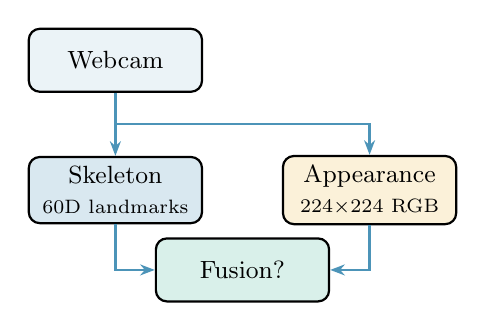
\begin{tikzpicture}[
                box/.style={draw, rounded corners, fill=primary!8, minimum width=2.2cm, minimum height=0.8cm, align=center, font=\small, thick},
                arrow/.style={-{Stealth[scale=0.8]}, thick, primary!70},
                node distance=0.8cm,
            ]
                \node[box] (cam) {Webcam};
                \node[box, below=of cam, fill=primary!15] (skel) {Skeleton\\{\scriptsize 60D landmarks}};
                \node[box, right=1cm of skel, fill=accent!15] (app) {Appearance\\{\scriptsize 224$\times$224 RGB}};
                \node[box, below=0.6cm of $(skel)!0.5!(app)$, fill=success!15] (fuse) {Fusion?};

                \draw[arrow] (cam.south) -- ++(0,-0.4) -| (skel.north);
                \draw[arrow] (cam.south) -- ++(0,-0.4) -| (app.north);
                \draw[arrow] (skel) |- (fuse);
                \draw[arrow] (app) |- (fuse);
            \end{tikzpicture}
        \end{column}
    \end{columns}
\end{frame}


% ======== 3. DATA & TWO MODALITIES ========
\begin{frame}{Dataset \& Two Feature Streams}
\begin{columns}[c]
\begin{column}{0.42\textwidth}
    \textbf{HaGRID v2 (Subset)}
    \begin{itemize}
        \item 23,850 samples, 13,250 subjects
        \item 5 classes: Pinch, Fist, Open, Frame, None
        \item \textbf{Person-aware} Group 5-Fold CV\\(no subject leakage)
    \end{itemize}
    
    \vspace{1em}
    \textbf{Two Modalities from One Camera:}
    \begin{itemize}
        \item \textcolor{primary}{\textbf{Skeleton:}} MediaPipe $\to$ 21~joints $\to$ normalized 60D vector
        \item \textcolor{accent}{\textbf{Appearance:}} YOLO crop $\to$ 224$\times$224 RGB
    \end{itemize}
\end{column}
\begin{column}{0.53\textwidth}
    \centering
    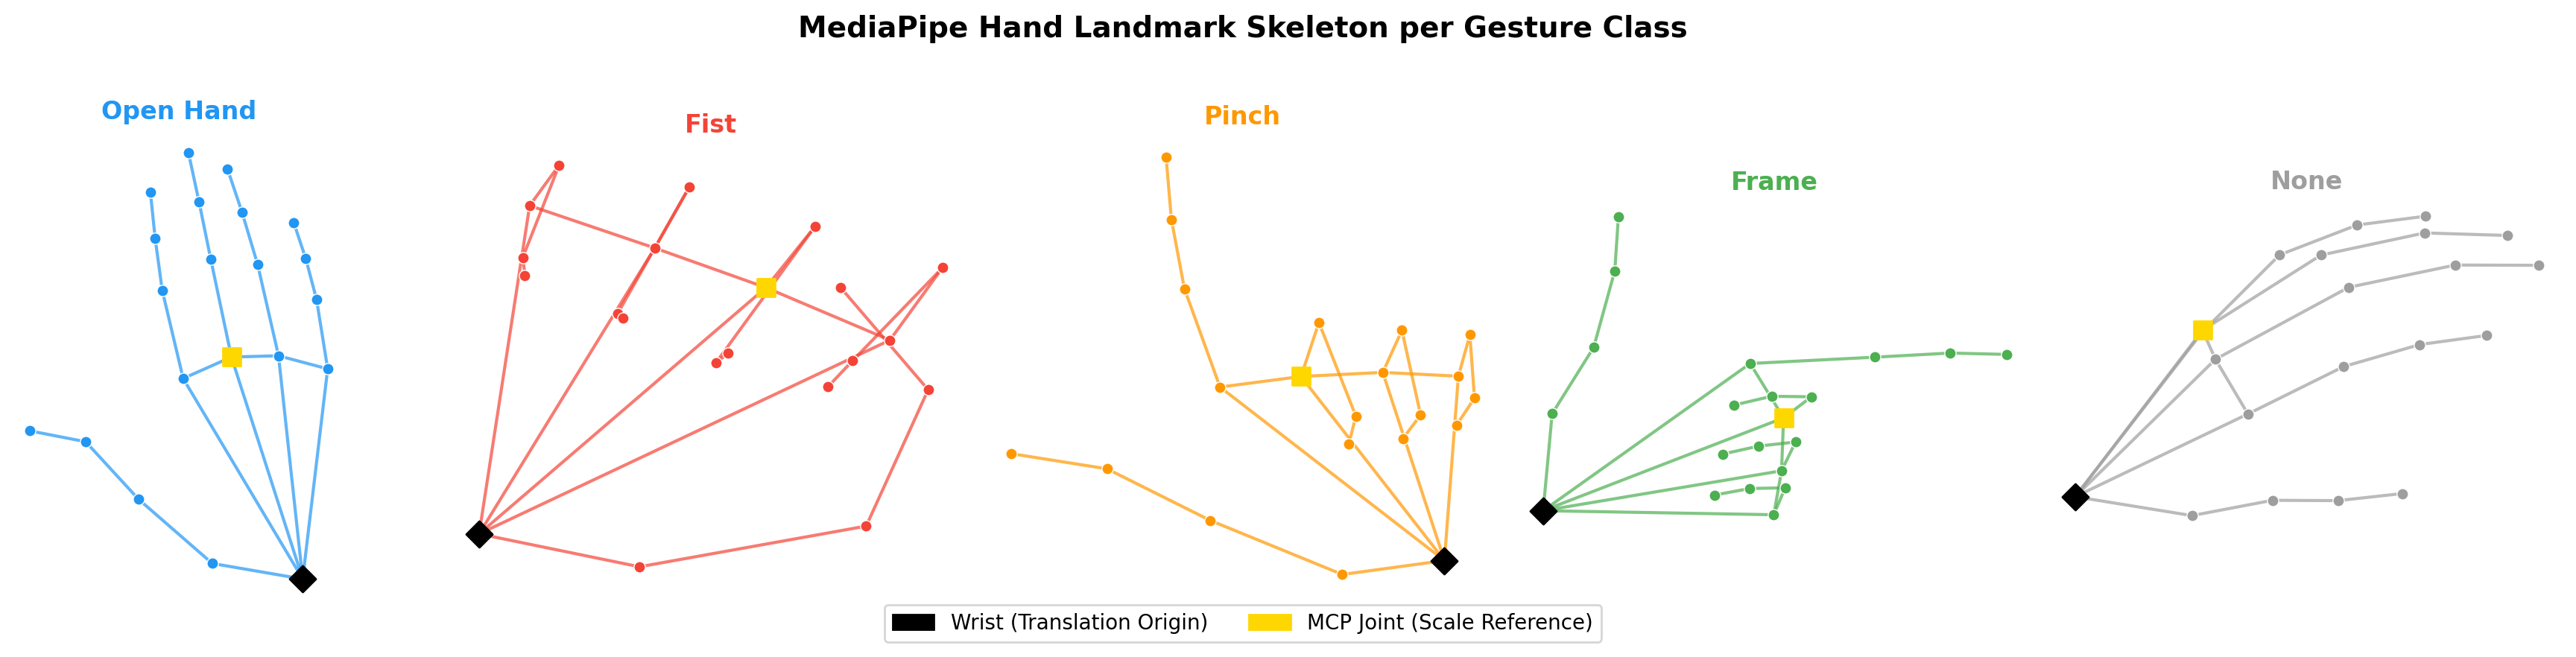
\includegraphics[width=0.95\textwidth]{landmark_skeleton_per_class.png}
    {\small \textit{Skeleton: geometrically distinct classes}}

    \vspace{0.8em}
    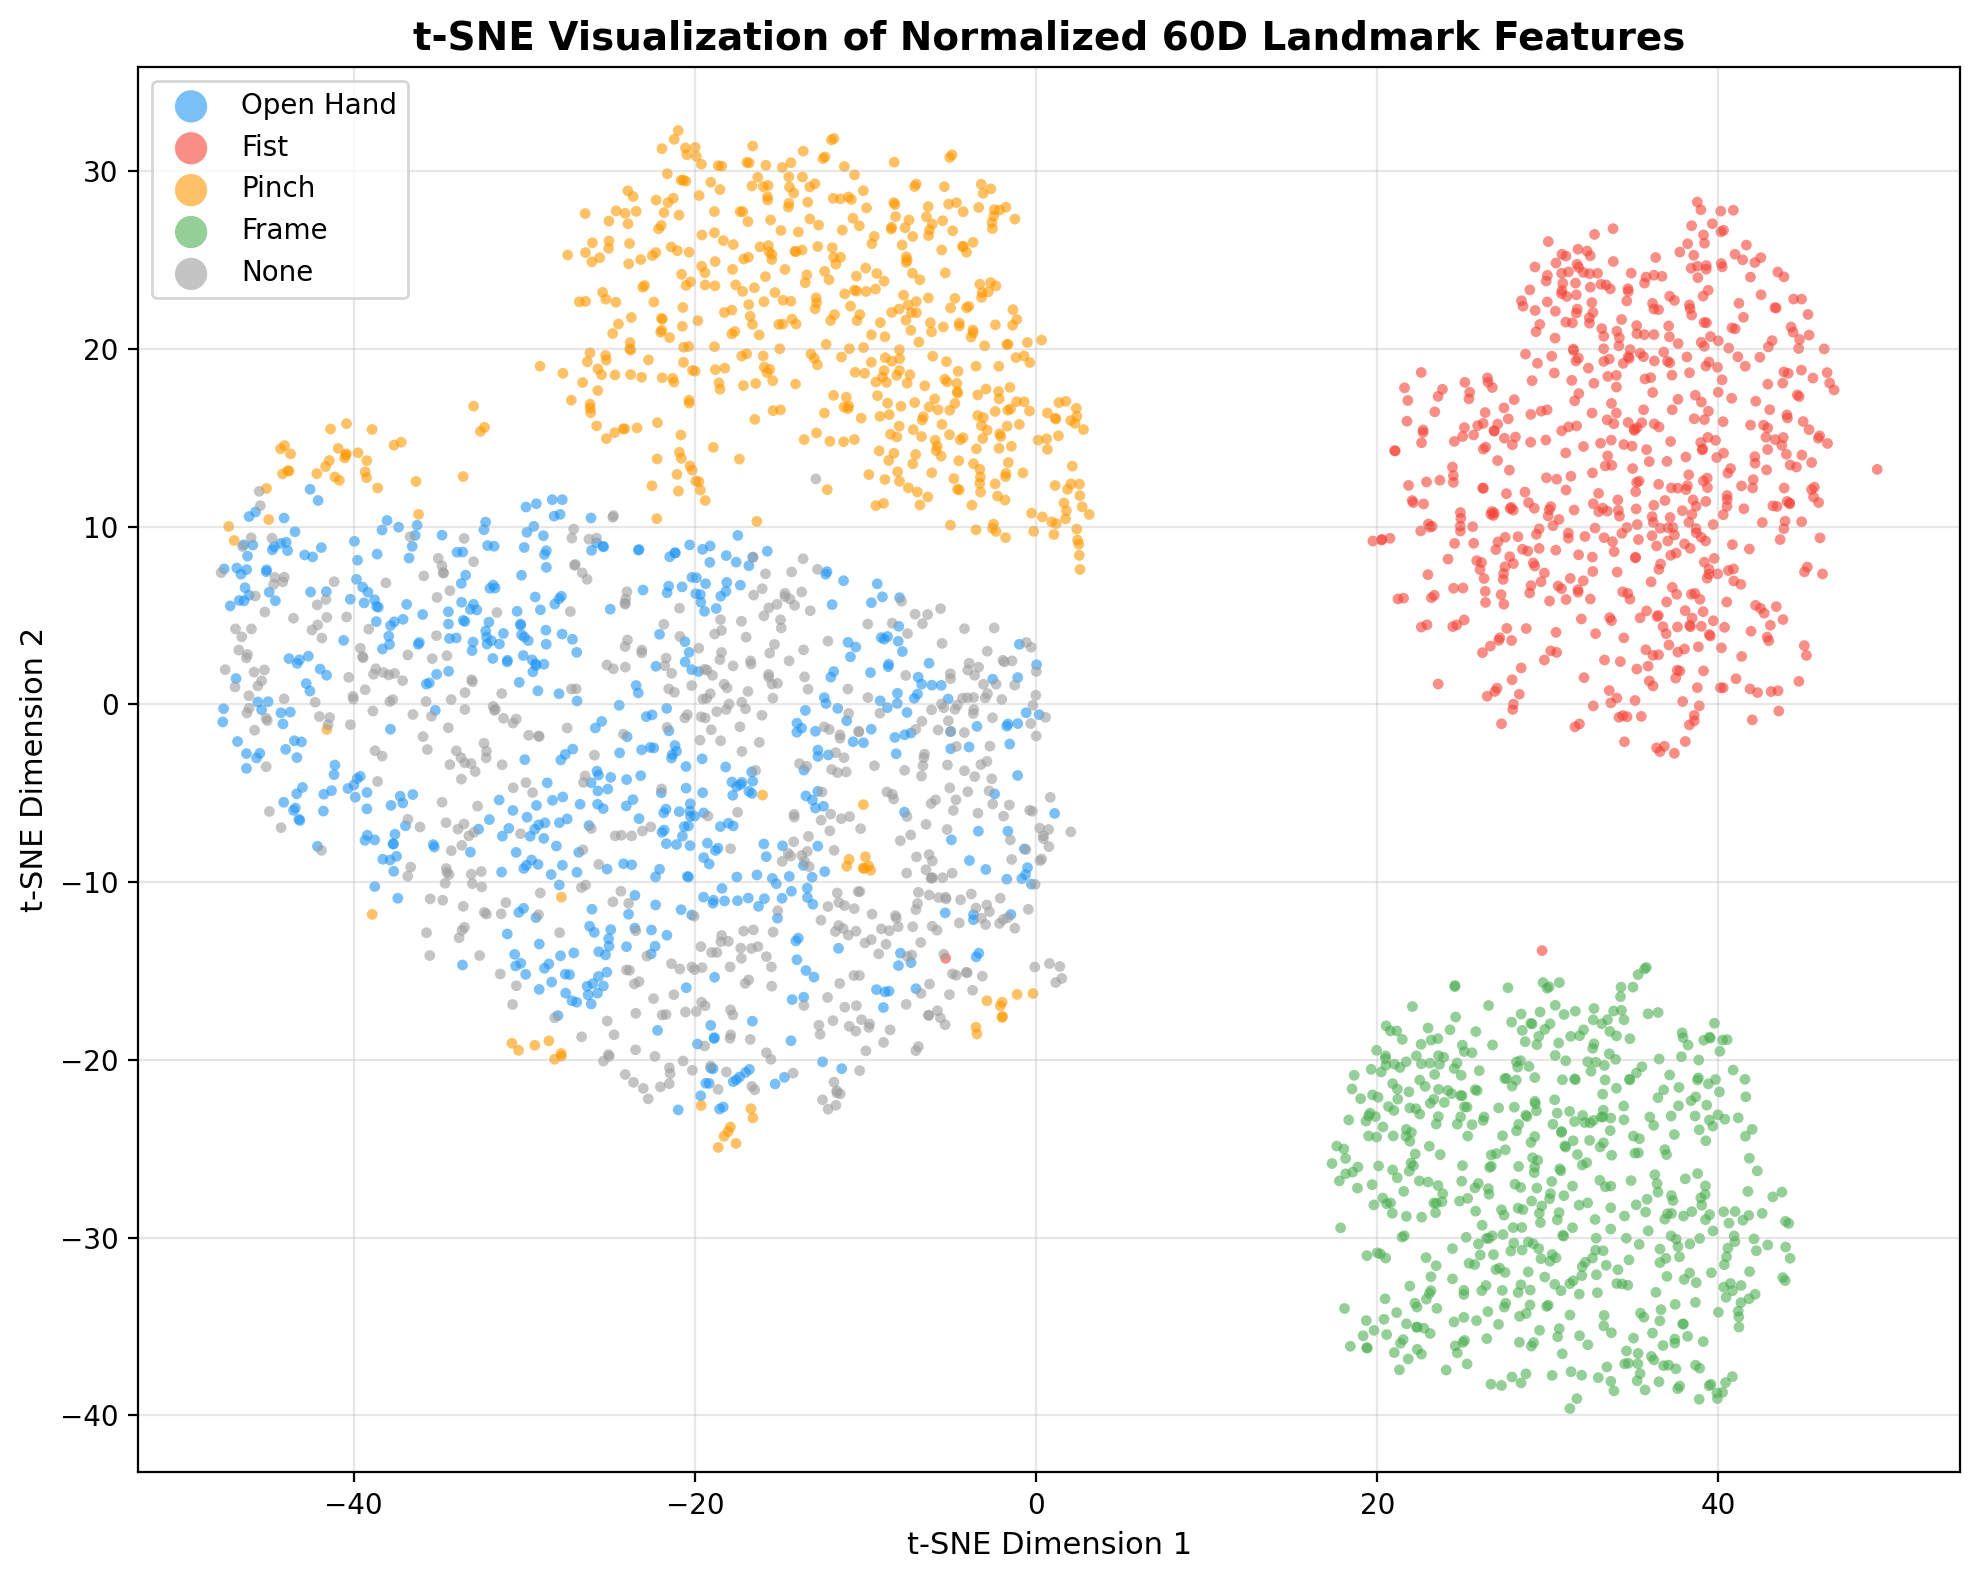
\includegraphics[width=0.75\textwidth]{tsne_feature_space.png}
    {\small \textit{t-SNE: already well-separated in 60D space}}
\end{column}
\end{columns}
\end{frame}


% ======== 4. METHODS & RESULTS ========
\begin{frame}{Methods \& Results}
\begin{columns}[T]
\begin{column}{0.52\textwidth}
    \vspace{0.5em}
    \textbf{Six methods, two modalities:}
    
    \vspace{0.5em}
    \resizebox{\textwidth}{!}{
    \begin{tabular}{llrrl}
    \toprule
    \textbf{Method} & \textbf{Modality} & \textbf{Acc} & \textbf{Params} & \textbf{Size} \\
    \midrule
    Heuristic & Skeleton & 1.0\% & $\sim$20 & 170 B \\
    Random Forest & Skeleton & 94.1\% & $\sim$100K & 8.6 MB \\
    \rowcolor{primary!12}
    \textbf{MLP} & \textbf{Skeleton} & \textbf{99.8\%} & \textbf{14.7K} & \textbf{227 KB} \\
    CNN & Appear. & 100.0\% & 1.5M & 0.3 MB \\
    YOLOv8n & Appear. & 99.5\%$^\dagger$ & 3.0M & 6.2 MB \\
    \rowcolor{success!10}
    \textbf{Fusion} & \textbf{Both} & \textbf{100.0\%} & --- & \textbf{0.5 MB} \\
    \bottomrule
    \end{tabular}
    }
    {\scriptsize $^\dagger$mAP@50 (detection metric)}
    
    \vspace{0.8em}
    \textbf{Person-aware Group 5-Fold CV}\\
    {\small 13,250 subjects $\times$ 5 folds\\= every person tested as ``unseen''}
\end{column}
\begin{column}{0.45\textwidth}
    \centering
    
\includegraphics[width=\textwidth]{accuracy_comparison.png}

    \vspace{0.3em}
    
\includegraphics[width=\textwidth]{per_class_f1_comparison.png}
    
    {\scriptsize Weakest: ``None'' (heterogeneous negatives)}
\end{column}
\end{columns}
\end{frame}


% ======== 5. KEY FINDING: CEILING EFFECT ========
\begin{frame}{Key Finding: The Ceiling Effect}
    \centering
    \vspace{1em}

    {\Large Both modalities \textbf{independently} achieve near-perfect accuracy.\\[0.3em]
    Fusion adds \textbf{zero measurable benefit}.}

    \vspace{2em}
    \begin{columns}[T]
    \begin{column}{0.45\textwidth}
        \textbf{Why this is a valid finding:}
        \begin{enumerate}
            \setlength\itemsep{0.6em}
            \item 5 gestures are \textbf{geometrically unambiguous}\\(fist $\neq$ open $\neq$ pinch)
            \item Person-aware CV: \textbf{zero identity leakage}
            \item 13,250 subjects, clean labels
        \end{enumerate}
    \end{column}
    \begin{column}{0.45\textwidth}
        \textbf{What this tells us:}
        \begin{enumerate}
            \setlength\itemsep{0.6em}
            \item \textbf{Task difficulty} is the dominant factor,\\not model capacity
            \item For simple vocabularies:\\single-modality \textbf{MLP suffices}
            \item Fusion value appears at harder tasks\\(full HaGRID: 18 classes, 95.5\% SOTA)
        \end{enumerate}
    \end{column}
    \end{columns}

    \vspace{1.5em}
    \begin{block}{}
        \centering
        \textbf{Practical answer:} Deploy a \textbf{227 KB MLP} on skeleton. It's enough.
    \end{block}
\end{frame}


% ======== 6. BEYOND CLASSIFICATION ========
\begin{frame}{Beyond Classification: Mathematical Interaction Model}
    \centering
    \vspace{0.3em}

    {\small 99.8\% accuracy $\neq$ usable control. Hand jitter $\to$ erratic cursor. Transient errors $\to$ dropped tiles.\\
    \textbf{Solution:} Adapt the directional threshold model from Huda et al. 2025 (wheelchair control).}

    \vspace{0.6em}
    \begin{columns}[c]
    \begin{column}{0.45\textwidth}
        \centering
        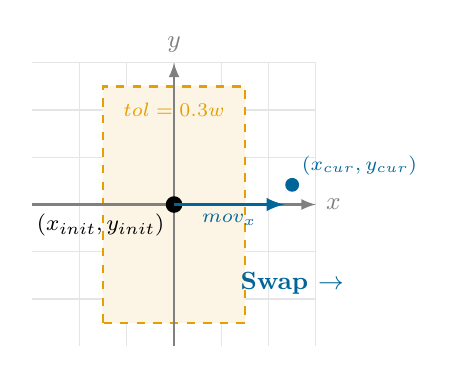
\begin{tikzpicture}[
            tol/.style={draw=accent, thick, dashed, fill=accent!10},
            axis/.style={-latex, thick, gray},
            move/.style={-latex, very thick, primary},
        ]
            % Background grid hint
            \draw[gray!20, step=0.6] (-1.8,-1.8) grid (1.8,1.8);
            
            % Tolerance zone
            \draw[tol] (-0.9, -1.5) rectangle (0.9, 1.5);
            \node[accent, font=\scriptsize] at (0, 1.2) {$tol = 0.3w$};
            
            % Axes
            \draw[axis] (-1.8, 0) -- (1.8, 0) node[right, font=\small] {$x$};
            \draw[axis] (0, -1.8) -- (0, 1.8) node[above, font=\small] {$y$};
            
            % Initial point
            \fill (0,0) circle (3pt) node[below left, font=\footnotesize] {$(x_{init}, y_{init})$};
            
            % Movement threshold arrows
            \draw[move] (0,0) -- (1.4, 0);
            \node[primary, font=\scriptsize, below] at (0.7, 0) {$mov_x$};
            
            % Current position
            \fill[primary] (1.5, 0.25) circle (2.5pt) node[above right, font=\scriptsize] {$(x_{cur}, y_{cur})$};
            
            % Label: Swipe Right
            \node[primary, font=\small\bfseries] at (1.5, -1.0) {Swap $\to$};
        \end{tikzpicture}
        
        \vspace{0.3em}
        {\scriptsize Huda et al.: wheelchair direction.\\Ours: puzzle tile swap.}
    \end{column}
    \begin{column}{0.5\textwidth}
        \small
        Let $\Delta x = x_{cur} - x_{init}$,\enspace $\Delta y = y_{cur} - y_{init}$
        
        \vspace{0.5em}
        \begin{tabular}{ll}
        \toprule
        \textbf{Action} & \textbf{Condition} \\
        \midrule
        Swap $\to$ & $\Delta x > mov_x$ \textbf{AND} $|\Delta y| < tol$ \\
        Swap $\leftarrow$ & $\Delta x < -mov_x$ \textbf{AND} $|\Delta y| < tol$ \\
        Swap $\uparrow$ & $\Delta y < -mov_y$ \textbf{AND} $|\Delta x| < tol$ \\
        Swap $\downarrow$ & $\Delta y > mov_y$ \textbf{AND} $|\Delta x| < tol$ \\
        \bottomrule
        \end{tabular}
        
        \vspace{0.8em}
        {\footnotesize
        $mov_{x,y} = 0.6 \times \text{tile\_size}$\\
        $tol = 0.3 \times \text{tile\_size}$\\[0.3em]
        Origin resets after each swap\\$\to$ continuous multi-step swiping.}
    \end{column}
    \end{columns}
\end{frame}


% ======== 7. CONCLUSION & LIMITATIONS ========
\begin{frame}{Conclusion \& Limitations}
    \vspace{0.5em}

    \begin{columns}[T]
    \begin{column}{0.55\textwidth}
        \textbf{Contributions:}
        \begin{enumerate}
            \setlength\itemsep{0.8em}
            \item \textbf{Multi-modal investigation:} Both skeleton (MLP, 99.8\%) and appearance (CNN, 100\%) independently saturate accuracy for 5 coarse gestures. Fusion adds no benefit --- a \textbf{ceiling effect} driven by task simplicity.

            \item \textbf{Mathematical interaction model:} Adapted from Huda et al. 2025 (wheelchair $\to$ puzzle) using $mov_x$, $mov_y$, $tol$ thresholds + 3-frame debounce + adaptive cursor.

            \item \textbf{Client-side deployment:} 227~KB MLP, 30+ FPS, zero server dependency.
        \end{enumerate}
    \end{column}
    \begin{column}{0.42\textwidth}
        \textbf{Limitations:}
        \begin{itemize}
            \setlength\itemsep{0.6em}
            \item 5 gestures are \textbf{trivially separable} --- fusion benefit expected at 18+ classes
            \item Interaction model parameters ($mov$, $tol$) are \textbf{fixed}, not user-calibrated
            \item No formal \textbf{user study} on task completion rate
        \end{itemize}

        \vspace{0.8em}
        \textbf{Future:}
        \begin{itemize}
            \item Extend to full HaGRID (18 classes)
            \item Per-user threshold calibration
            \item Formal usability study
        \end{itemize}
    \end{column}
    \end{columns}
\end{frame}


% ======== 8. THANK YOU ========
\begin{frame}[plain]
    \vfill
    \centering
    {\Huge\textcolor{primary}{Thank You}}

    \vspace{1em}
    {\large Questions \& Game Demo}

    \vspace{2em}
    {\small Hieu Dinh $\cdot$ Nhat Anh $\cdot$ Quoc Anh}
    \vfill
\end{frame}


% ================================================================
% BACKUP SLIDES (for Q\&A)
% ================================================================
\appendix

\begin{frame}[noframenumbering]{Backup: Confusion Matrices}
\begin{columns}[c]
\begin{column}{0.48\textwidth}
    \centering
    {\textbf{Random Forest (94\%)}}\\[0.3em]
    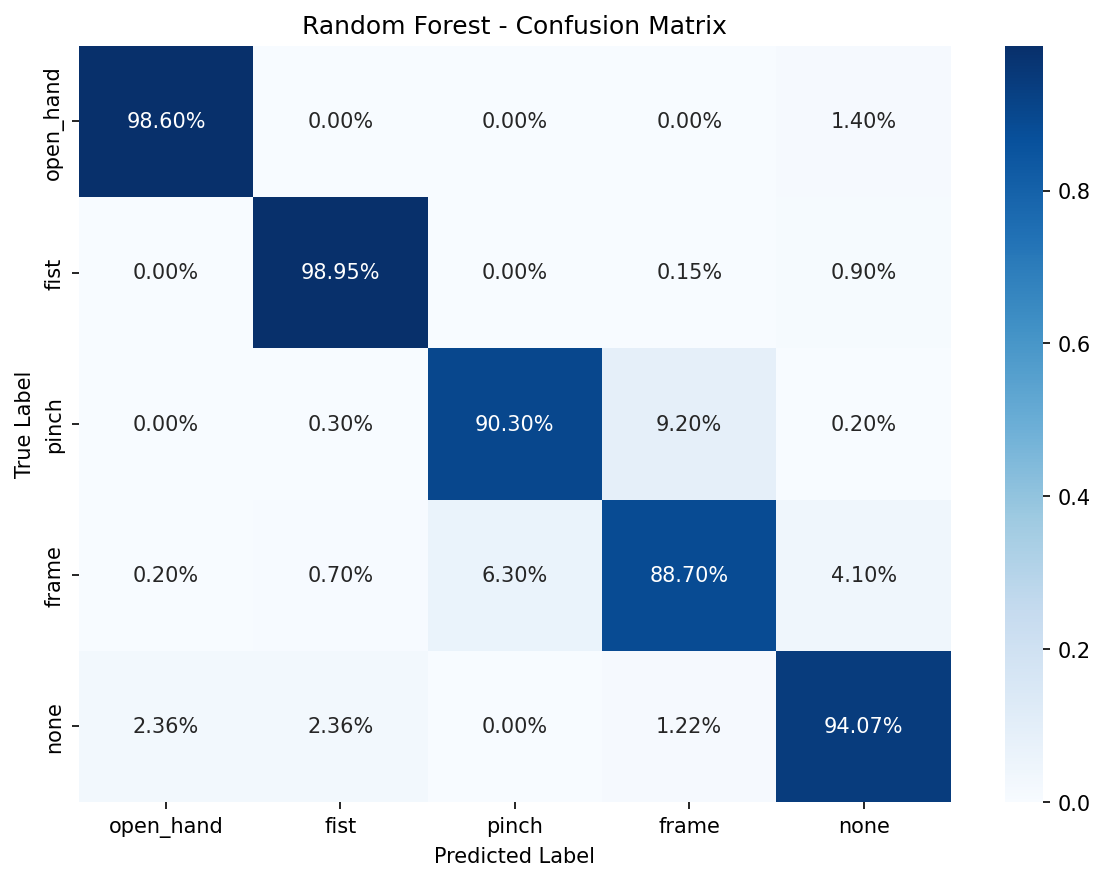
\includegraphics[width=\textwidth]{rf_confusion_matrix.png}
    {\small Frame $\leftrightarrow$ None confusion}
\end{column}
\begin{column}{0.48\textwidth}
    \centering
    {\textbf{MLP (99.8\%)}}\\[0.3em]
    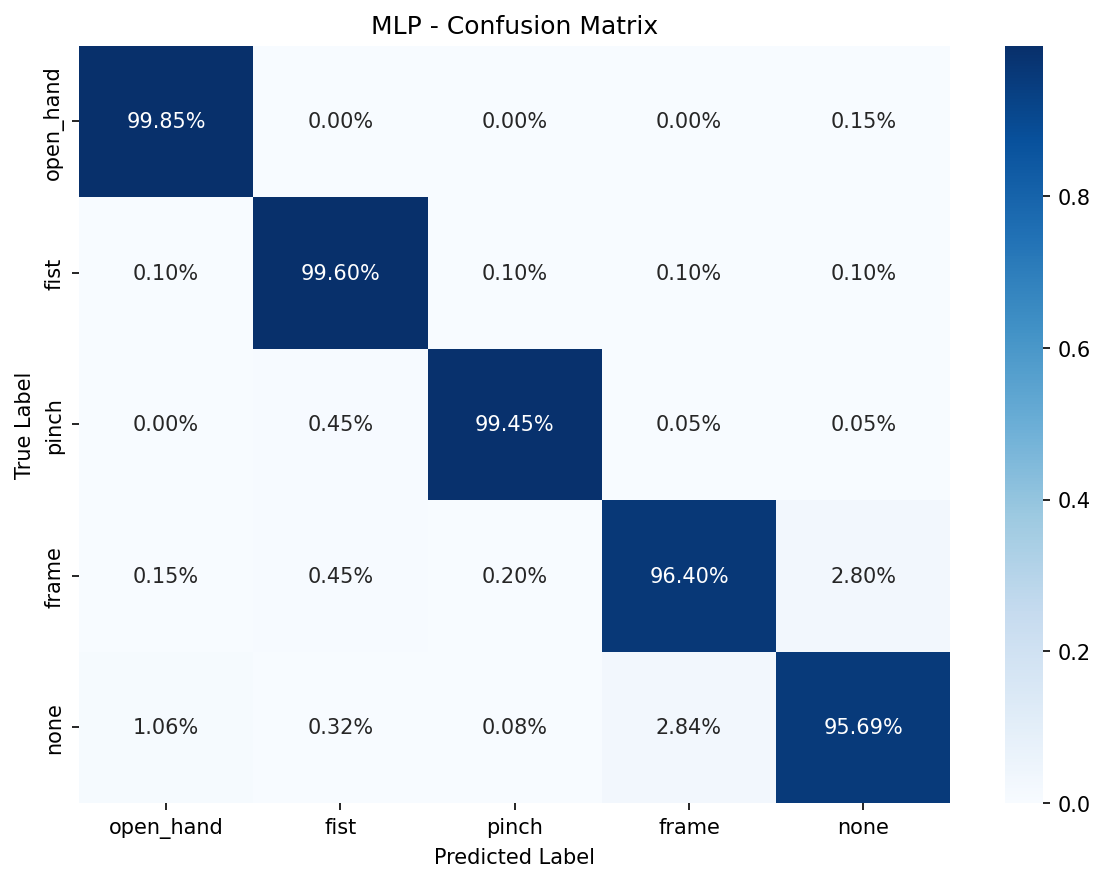
\includegraphics[width=\textwidth]{mlp_confusion_matrix.png}
    {\small Full 60D resolves it}
\end{column}
\end{columns}
\end{frame}

\begin{frame}[noframenumbering]{Backup: YOLO Detection Results}
    \centering
    \vspace{1em}
    
    \textbf{YOLOv8n} --- simultaneous detection + classification
    
    \vspace{1em}
    \begin{tabular}{lr}
    \toprule
    \textbf{Metric} & \textbf{Score} \\
    \midrule
    mAP@50 & 99.5\% \\
    mAP@50:95 & 90.7\% \\
    Parameters & 3.0M \\
    Model size & 6.2 MB \\
    \bottomrule
    \end{tabular}
    
    \vspace{1.5em}
    {\small Different task than classification (includes localization).\\
    Useful when hand bounding box is unknown at inference.\\
    \textbf{But:} 20$\times$ larger than MLP --- overkill when MediaPipe provides landmarks.}
\end{frame}

\begin{frame}[noframenumbering]{Backup: SOTA Context}
    \centering
    \vspace{1em}
    
    \textbf{HaGRID baselines} (full 18-class set, 554K images):
    
    \vspace{0.8em}
    \begin{tabular}{llr}
    \toprule
    \textbf{Method} & \textbf{Params} & \textbf{F1} \\
    \midrule
    SSDLite+MobileNetV3-S & --- & 57.7 \\
    SSDLite+MobileNetV3-L & --- & 71.6 \\
    ResNet-18 & 11M & 89.6 \\
    ResNeXt-101 & 44M & 87.0 \\
    ResNet-152 & 60M & 95.5 \\
    \midrule
    \textbf{Ours: MLP on 5 classes} & \textbf{14.7K} & \textbf{99.8} \\
    \bottomrule
    \end{tabular}
    
    \vspace{1em}
    {\small Not directly comparable (5 vs 18 classes), but shows:\\a tiny MLP saturates a simple subset of the same dataset.}
\end{frame}

\begin{frame}[noframenumbering]{Backup: Frame Gesture \& Deployment Differences}
\begin{columns}[T]
\begin{column}{0.48\textwidth}
    \textbf{Benchmarking vs.\ Deployed System}

    \vspace{0.5em}
    \begin{tabular}{lll}
    \toprule
    \textbf{Aspect} & \textbf{Benchmark} & \textbf{Deployed} \\
    \midrule
    Classifier & MLP (5-class) & MLP (4-class) \\
    Frame detect & MLP & 2-hand heuristic \\
    CNN & Evaluated & Optional \\
    Fusion & Evaluated & Not used \\
    \bottomrule
    \end{tabular}

    \vspace{0.8em}
    {\small The 99.8\% accuracy is from the 5-class MLP in the benchmarking study. The deployed system uses a simpler, more robust configuration.}
\end{column}
\begin{column}{0.48\textwidth}
    \textbf{Why bypass MLP for ``frame''?}

    \vspace{0.5em}
    \begin{itemize}
        \setlength\itemsep{0.5em}
        \item ``Frame'' = two hands forming rectangle
        \item MediaPipe reliably detects 2 hands
        \item Two-hand presence is the \textbf{defining property} of the gesture
        \item More robust than classifying from a single-hand crop
    \end{itemize}

    \vspace{0.5em}
    {\small This is a practical deployment optimization, not a limitation of the classifier.}
\end{column}
\end{columns}
\end{frame}

\end{document}
